%%%%%%%%%%%%%%%%%%%%%%%%%%%%%%%%%%%%%%%%%%%%%%%%%%%%%%%%%%%%%%%%%%%%%%%%%%%%
%% Author template for INFORMS Journal on Data Science (ijds) [interim solution; new styles under construction]
%% Mirko Janc, Ph.D., INFORMS, mirko.janc@informs.org
%% ver. 0.91, March 2015 - updated November 2020 by Matthew Walls, matthew.walls@informs.org
%% Adapted for rticles by Rob J Hyndman Rob.Hyndman@monash.edu. Dec 2021
%%%%%%%%%%%%%%%%%%%%%%%%%%%%%%%%%%%%%%%%%%%%%%%%%%%%%%%%%%%%%%%%%%%%%%%%%%%%
\documentclass[,,nonblindrev]{informs}

\OneAndAHalfSpacedXI
%%\OneAndAHalfSpacedXII % Current default line spacing
%%\DoubleSpacedXII
%%\DoubleSpacedXI

%% BEGIN MY ADDITIONS %%
\usepackage{hyperref}

% tightlist command for lists without linebreak
\providecommand{\tightlist}{%
  \setlength{\itemsep}{0pt}\setlength{\parskip}{0pt}}



\usepackage{booktabs}
\usepackage{tabularx}
\usepackage{graphicx}
\usepackage{tikz}
\usepackage{siunitx}
\usepackage{tablefootnote}
\usepackage{longtable}
\usepackage{threeparttable}
\usepackage{natbib}
\usepackage{caption}

%% END MY ADDITIONS %%


% Natbib setup for author-year style
\usepackage{natbib}
 \bibpunct[, ]{(}{)}{,}{a}{}{,}%
 \def\bibfont{\small}%
 \def\bibsep{\smallskipamount}%
 \def\bibhang{24pt}%
 \def\newblock{\ }%
 \def\BIBand{and}%


%% Setup of theorem styles. Outcomment only one.
%% Preferred default is the first option.
\TheoremsNumberedThrough     % Preferred (Theorem 1, Lemma 1, Theorem 2)
%\TheoremsNumberedByChapter  % (Theorem 1.1, Lema 1.1, Theorem 1.2)
\ECRepeatTheorems

%% Setup of the equation numbering system. Outcomment only one.
%% Preferred default is the first option.
\EquationsNumberedThrough    % Default: (1), (2), ...
%\EquationsNumberedBySection % (1.1), (1.2), ...

% For new submissions, leave this number blank.
% For revisions, input the manuscript number assigned by the on-line
% system along with a suffix ".Rx" where x is the revision number.
\MANUSCRIPTNO{}

%%%%%%%%%%%%%%%%
\begin{document}
%%%%%%%%%%%%%%%%

% Outcomment only when entries are known. Otherwise leave as is and
%   default values will be used.
%\setcounter{page}{1}
%\VOLUME{00}%
%\NO{0}%
%\MONTH{Xxxxx}% (month or a similar seasonal id)
%\YEAR{0000}% e.g., 2005
%\FIRSTPAGE{000}%
%\LASTPAGE{000}%
%\SHORTYEAR{00}% shortened year (two-digit)
%\ISSUE{0000} %
%\LONGFIRSTPAGE{0001} %
%\DOI{10.1287/xxxx.0000.0000}%

% Author's names for the running heads
% Sample depending on the number of authors;
\RUNAUTHOR{%
Jameson, Saghafian, Huckman
 and Hodgson
}
% \RUNAUTHOR{Jones and Wilson}
% \RUNAUTHOR{Jones, Miller, and Wilson}
% \RUNAUTHOR{Jones et al.} % for four or more authors
% Enter authors following the given pattern:
%\RUNAUTHOR{}

\RUNTITLE{To Batch or Not to Batch: Test-Ordering Variability in the ED}

\TITLE{To Batch or Not to Batch: Test-Ordering Variability in the ED}

\ARTICLEAUTHORS{%
\AUTHOR{Jacob Jameson}
\AFF{Interfaculty Initiative in Health Policy, Harvard
University, \EMAIL{\href{mailto:jacobjameson@g.harvard.edu}{\nolinkurl{jacobjameson@g.harvard.edu}}}}

\AUTHOR{Soroush Saghafian}
\AFF{Kennedy School of Government, Harvard
University, \EMAIL{\href{mailto:soroush_saghafian@hks.harvard.edu}{\nolinkurl{soroush\_saghafian@hks.harvard.edu}}}}

\AUTHOR{Robert Huckman}
\AFF{Harvard Business
School, \EMAIL{\href{mailto:rhuckman@hbs.edu}{\nolinkurl{rhuckman@hbs.edu}}}}

\AUTHOR{Nicole Hodgson}
\AFF{Mayo
Clinic, \EMAIL{\href{mailto:Hodgson.Nicole@mayo.edu}{\nolinkurl{Hodgson.Nicole@mayo.edu}}}}

%
}

\ABSTRACT{We use practice variation across physicians to uncover the
role of test-ordering on care delivery in the ED. Using records of over
45,000 Mayo Clinic emergency department visits\ldots{}}

\KEYWORDS{Emergency Department, Operational Effeciency, Diagnostic
Testing}

\maketitle


\hypertarget{sec:I}{%
\section{Introduction}\label{sec:I}}

Healthcare delivery, particularly in the emergency department (ED),
requires a delicate balance between ensuring optimal patient outcomes
and optimizing resource utilization. Achieving these twin goals
necessitates timely and accurate diagnosis, which enables prompt and
appropriate treatment, improving patient prognosis and reducing the
likelihood of adverse events. Efficient patient discharge from the ED is
crucial for alleviating overcrowding, a severe issue associated with
higher complication rates and increased mortality \citet{bernstein2009}.
In this complex environment, the availability and performance of
diagnostic tests, especially imaging studies, play a pivotal role in
shaping both patient care and operational efficiency \citet{naseim2015}.

A critical question in ED management pertains to whether physicians
should batch order diagnostic imaging tests or order them sequentially.
This decision represents a fundamental tradeoff between potentially
reducing patient length of stay and risking over-testing. Batch
ordering, where multiple imaging tests are ordered simultaneously, may
expedite the diagnostic process but can lead to unnecessary tests,
increased costs, patient anxiety, and potential harm from follow-up of
false-positive results \citet{koch2018}. Conversely, a more sequential
approach might reduce unnecessary testing but could extend a patient's
time in the ED, potentially contributing to overcrowding. Striking the
right balance between comprehensive evaluation and efficient resource
use is crucial, yet research on optimal test ordering strategies in the
ED remains limited \citet{saghafian2015}.

In this paper, we leverage data from over 45,000 ED patient visits to
quantify the benefits and consequences of batching versus sequentially
ordering diagnostic imaging tests. Our focus on imaging tests is
particularly relevant given their significant impact on patient flow,
resource utilization, and potential health risks from radiation
exposure. We employ an empirical strategy that exploits the random
assignment of patients to ED physicians who differ in their propensity
to batch-order imaging tests. This quasi-experimental design allows us
to overcome potential selection bias and move closer to identifying the
causal impact of batch ordering on key outcomes such as patient length
of stay, resource utilization, and the likelihood of return visits.

To capture physician tendencies towards batch ordering, we introduce a
novel measure using a leave-out, residualized approach based on each
physician's historical ordering patterns for all other patients seen
during the study period. This tendency measure strongly predicts actual
batch ordering behavior while remaining uncorrelated with patient and ED
visit characteristics, providing a robust instrument for our analysis.
Our findings reveal significant practice variation among physicians and
demonstrate substantial impacts on ED operations and patient care
trajectories.

We begin by evaluating the reduced-form effects of ED provider
batch-ordering tendency on downstream patient outcomes and ED turnaround
time. Our results indicate that practice variation, as captured by
physician batch-ordering tendency, has large and significant
consequences. For instance, being treated by a provider in the top
decile of the batching tendency distribution, compared to one in the
bottom decile, results in additional diagnostic imaging tests per 100
patient encounters, even after controlling for the physician's
underlying propensity to test. This variation in practice patterns
raises important questions about the optimal use of diagnostic resources
in emergency care settings.

To address potential confounding factors, we employ a placebo exercise
to demonstrate that the observed effects are primarily due to batching
behavior rather than other aspects of physician care that might
correlate with batching tendency. We find no significant effects of
physician batch tendency on key outcomes for a ``placebo sample'' of
patients visiting the ED for conditions that rarely result in batched
orders. This strengthens our confidence in the specificity of the
batching effect on patient outcomes and resource utilization.

Our research design closely approximates a randomized controlled trial
that assigns patients to batch-ordering or sequential-ordering arms,
leveraging the unique features of the ED setting. In this environment,
patients have no discretion over provider selection, and in our specific
ED, the random assignment of patients to physicians further mitigates
selection issues. The wide variation in batch-ordering practices among
physicians within the same hospital, despite following identical
guidelines, provides the necessary variation for our analysis. Moreover,
the typically short, one-off nature of ED patient-physician interactions
constrains decision-making to a more limited, observable set of choices
compared to other healthcare settings.

By exploiting this practice variation in ED settings, we aim to isolate
the impact of test batching from other potential channels that might
influence length of stay and patient outcomes in different healthcare
contexts. This approach allows us to more accurately identify the causal
impact of batch-ordering diagnostic imaging tests on patient outcomes
and resource utilization. Importantly, our study examines batching
decisions made within the bounds of normal clinical judgment and
practice norms, rather than focusing on deviations from clinical
guidelines or instances of substandard care.

The implications of this research extend beyond academic interest,
offering potential insights for ED management, healthcare policy, and
the design of clinical decision support systems. Understanding the true
impacts of batch ordering practices could inform more efficient resource
allocation strategies, improve patient flow, and ultimately enhance the
quality of emergency care delivery. The remainder of this paper is
structured as follows: The next section describes our data source and
outlines the baseline sample. Section II describes the theoretical and
conceptual model. Section IV details our empirical strategy and its
accompanying identifying assumptions. Section V presents our results,
including both reduced-form effects and instrumental variable analyses.
Section V also discusses the implications of our findings for
batch-ordering policies and ED management. The final section concludes
with a summary of our contributions and directions for future research.

\hypertarget{theoretical-model}{%
\section{Theoretical Model}\label{theoretical-model}}

Emergency departments (EDs) are complex environments where critical
decisions about patient care must be made rapidly and under conditions
of uncertainty. Our theoretical model aims to capture the nuanced
dynamics of diagnostic decision-making in this high-stakes setting, with
a particular focus on the practice of batch ordering imaging tests.

In a typical ED scenario, patients arrive with varying levels of acuity
and a wide range of presenting symptoms. Upon arrival, each patient
\(i\) is assigned to a physician \(j\), often based on availability
rather than specific matching criteria. The physician's primary task is
to diagnose and treat the patient efficiently and effectively, a process
that frequently involves ordering diagnostic tests, including imaging
studies.

Central to our model is the concept of the patient's underlying
condition, denoted by \(\tau_i\). This represents the true state of the
patient's health, which is initially unknown to the treating physician.
The physician's goal is to uncover \(\tau_i\) as accurately and quickly
as possible to provide appropriate care. However, the path to this
discovery is not straightforward and involves critical decisions about
diagnostic testing.

The physician's approach to ordering tests is influenced by various
factors, including their individual tendencies and experiences. We
represent this as \(Z_j\), the physician's propensity to batch order
tests. This tendency can be thought of as a stable characteristic of the
physician, shaped by their training, past experiences, and personal
practice style. The decision to batch order tests for a given patient,
represented by \(X_{ij}\), is a function of both the physician's
tendency \(Z_j\) and the specifics of the patient's presentation. Batch
ordering involves requesting multiple imaging tests simultaneously,
rather than in a sequential manner. This decision has cascading effects
on the patient's journey through the ED.

\begin{figure}[h]
  \centering
  \caption{Conceptual Model}
  \label{fig:dag}
  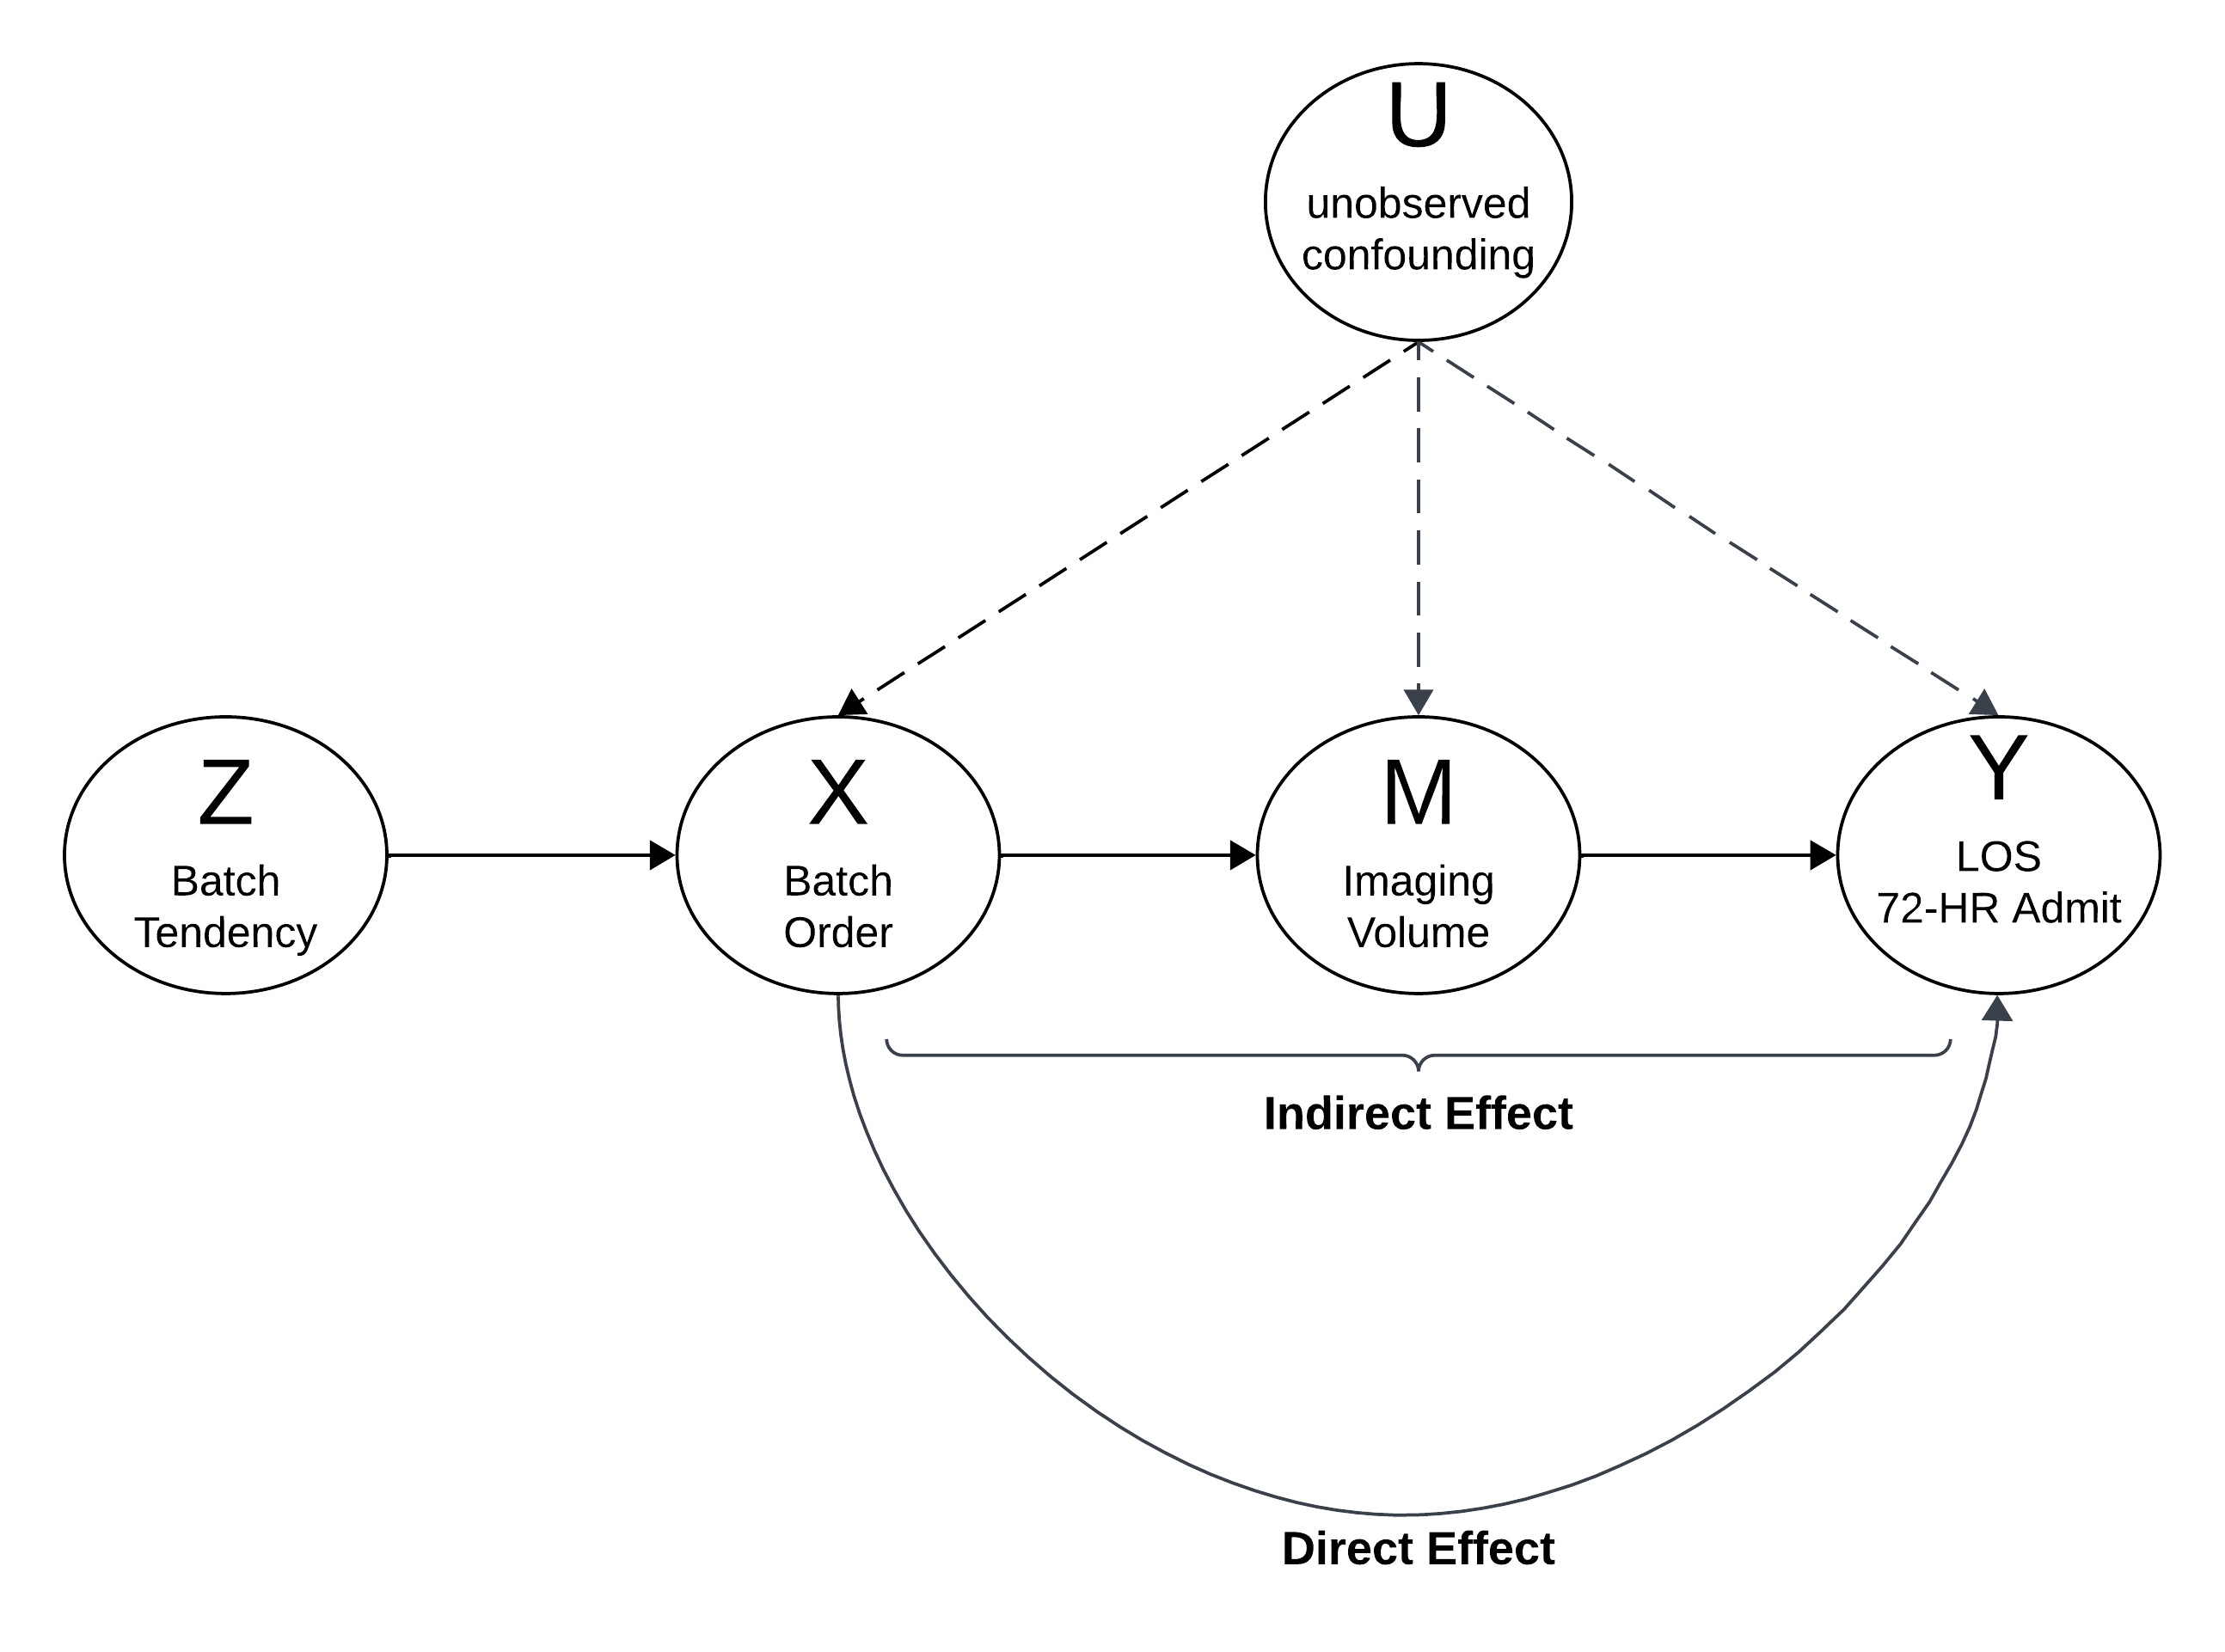
\includegraphics[width=4.25in]{model.png}
  \begin{tablenotes}
    \small
    \item \textit{Figure \ref{fig:dag} illustrates the causal relationships between physician tendency, batch ordering decision, test volume, and patient outcomes.}
  \end{tablenotes}
\end{figure}

As illustrated in Figure \ref{fig:dag}, when a physician chooses to
batch order (\(X_{ij} = 1\)), it directly influences the total volume of
imaging tests performed, \(M_{ij}\). Our model posits two key mechanisms
for this relationship:

\begin{enumerate}
  \item Precautionary ordering: In the face of diagnostic uncertainty, physicians may opt for a comprehensive initial workup, potentially including tests that might not have been ordered in a sequential approach.
  \item Reduced information gain: By ordering tests simultaneously, physicians forego the opportunity to use the results of initial tests to inform the necessity of subsequent ones. This can lead to a higher overall test volume compared to a sequential approach where each test order is informed by preceding results.
\end{enumerate}

The total volume of tests, \(M_{ij}\), in turn, impacts key patient
outcomes, \(Y_{ij}\), particularly length of stay (LOS) and the
probability of a 72-hour return visit with admission. The relationship
between test volume and these outcomes is complex. On one hand, more
tests generally require more time, potentially increasing LOS. However,
if the physician's initial diagnostic uncertainty is high, ordering more
tests upfront might expedite the diagnostic process and lead to quicker
treatment decisions.

Importantly, our model also allows for a direct effect of the batch
ordering decision on outcomes, independent of its effect through test
volume. This direct effect could represent, for example, the efficiency
gains from parallel processing of multiple tests, which might reduce LOS
even as the total number of tests increases. The model acknowledges the
presence of unobserved confounding factors, \(U_{ij}\), which might
influence both the decision to batch order and patient outcomes. These
could include factors like the physician's assessment of the patient's
condition severity or subtle clinical cues not captured in standard
data.

To formalize these relationships, we express them mathematically as
follows:

\begin{equation}
p(X_{ij}|Z_j) = f(Z_j, U_{ij})
\end{equation}

\begin{equation}
M_{ij} = g(X_{ij}, U_{ij})
\end{equation}

\begin{equation}
Y_{ij} = h(X_{ij}, M_{ij}, U_{ij})
\end{equation}

To address potential endogeneity, our empirical strategy leverages the
physician's general tendency to batch order, \(Z_j\), as an instrument
for the actual batching decision, \(X_{ij}\). This approach allows us to
estimate the causal effects of batch ordering on test volume and patient
outcomes, even in the presence of unobserved confounders.

Our empirical analysis focuses on estimating these key relationships:

\begin{enumerate}
  \item The effect of physician tendency on batching decisions: $\frac{\partial X_{ij}}{\partial Z_j}$
  \item The effect of batching on test volume: $\frac{\partial M_{ij}}{\partial X_{ij}}$
  \item The total effect of batching on patient outcomes: $\frac{\partial Y_{ij}}{\partial X_{ij}}$
\end{enumerate}

In summary, our theoretical model provides a framework for understanding
the complex decision-making process in ED diagnostic testing. It
highlights the potential trade-offs involved in batch ordering --
between comprehensive initial assessment and efficient resource use,
between rapid testing and informed sequential decision-making. By
formalizing these relationships, we set the stage for our empirical
analysis, which aims to quantify these effects and provide insights for
optimizing ED operations and patient care.

\hypertarget{sec:II}{%
\section{Data and Definitions}\label{sec:II}}

Our study was conducted in the Emergency Department (ED) of the Mayo
Clinic of Arizona, a tertiary care hospital without obstetrical
services, an inpatient pediatrics unit, or a trauma designation. During
the study period, the ED recorded approximately 43,000 visits per year,
managed across 26 treatment rooms and up to 9 hallway spaces. The
department is exclusively staffed by board-eligible or board-certified
emergency physicians (EPs), with rotating residents overseeing about
10\% of patient volume. Physicians operate in a unique workflow that
includes staggered 8.5-hour shifts and a rotational patient assignment
system, minimizing potential selection bias in patient encounters.

We conducted a retrospective review of comprehensive ED operational data
from 10/6/2018 through 12/31/2019, coinciding with the initiation of a
new electronic medical record. The dataset includes detailed patient
demographics, chief complaints, vital signs, emergency severity index
(ESI), length of stay (LOS), and resource utilization metrics. This
period was chosen to provide a robust data set while excluding the
influence of the coronavirus pandemic.

\hypertarget{sample-construction-and-summary-statistics}{%
\subsection{Sample Construction and Summary
Statistics}\label{sample-construction-and-summary-statistics}}

Our research design focuses on adult visits to the Mayo Clinic of
Arizona ED. From an initial dataset of approximately 48,000 visits
during the study period, we applied several exclusion criteria to
improve statistical power and ensure the validity of our physician batch
tendency instrument. We excluded encounters with rare chief complaints
(fewer than 1000 total encounters) and complaints where batch ordering
occurs in less than 5\% of cases. Examples of excluded complaints
include Upper Respiratory Symptoms and Urinary Complaints. This
exclusion strategy is unlikely to introduce selection bias as long as
physician test batching tendency is not strongly correlated with
diagnosing behavior across broad complaint categories. To estimate a
precise measure of physician-level batch tendency, we further restricted
our sample to encounters involving full-time physicians who treat over
500 ED cases per year. These criteria resulted in a final analytical
sample of 16,361 patient encounters.

Table \ref{tab:summary_statistics} provides a comprehensive overview of
ED characteristics, patient demographics, and medical tests in our study
site. The ED manages an average volume of 24.3 patients, indicating a
significant yet manageable workload. The patient population exhibits a
range of critical conditions, with 18.8\% presenting as tachycardic,
9.51\% as tachypneic, 2.43\% with fever, and 1.57\% as hypotensive.
Diagnostic procedures in our sample heavily rely on laboratory tests,
used in 78.5\% of encounters. Imaging plays a crucial role, with X-rays
ordered in 48.1\% of visits, non-contrast CT scans in 23.1\%, and
contrast CT scans in 20.5\%. Ultrasounds are used in 12.5\% of
encounters. Notably, 6.32\% of visits involve batch ordering of imaging
tests, a key focus of our study.

\begin{table}[ht]
\centering
\caption{Summary Statistics of Emergency Department Encounters}
\label{tab:summary_statistics}
\begin{tabular}{p{10.5cm}cccc}
\toprule
\textbf{} & \textbf{Mean} & \textbf{Q1} & \textbf{Median} & \textbf{Q3} \\
\midrule
\multicolumn{5}{l}{\textbf{Emergency Department Characteristics}} \\
Patients in ED & 24.3 & 16 & 25 & 33 \\
\\
Tachycardic & 0.188 & & & \\
Tachypneic & 0.095 & & & \\
Febrile & 0.024 & & & \\
Hypotensive & 0.016 & & & \\
\\
ESI & 2.74 & 2 & 3 & 3 \\
\\
Complaint: Abdominal Complaints & 0.169 & & & \\
Complaint: Extremity Complaints & 0.143 & & & \\
Complaint: Chest Pain & 0.096 & & & \\
Complaint: Neurological Issue & 0.095 & & & \\
Complaint: Gastrointestinal Issues & 0.090 & & & \\
\midrule
\multicolumn{5}{l}{\textbf{Patient Characteristics}} \\
Arrival Age & 58.3 & 44 & 61 & 75 \\
\\
Race: White & 0.886 & & & \\
Race: Black & 0.041 & & & \\
Race: Asian & 0.030 & & & \\
\\
Gender: Female & 0.545 & & & \\
\midrule
\multicolumn{5}{l}{\textbf{Tests}} \\
X-Ray & 0.481 & & & \\
Ultrasound & 0.125 & & & \\
Non-Contrast CT & 0.231 & & & \\
Contrast CT & 0.205 & & & \\
Lab & 0.785 & & & \\
\\
Imaging Tests were Batch Ordered & 0.063 & & & \\
\bottomrule
\end{tabular}
\begin{tablenotes}
\small
\item \textit{This table reports summary statistics for the baseline sample of emergency department visits during the study period described in the text. Vital signs were categorized as follows: tachycardia (pulse more significant than $100$), tachypnea (respiratory rate greater than $20$), fever (temperature greater than $38^\circ C$), and hypotension (systolic blood pressure less than $90$).}
\end{tablenotes}
\end{table}

This sample composition and these descriptive statistics provide
essential context for our subsequent analyses of batch ordering
practices and their impacts on ED efficiency and patient outcomes. The
diversity in patient characteristics, presenting complaints, and
diagnostic approaches underscores the complexity of ED operations and
the potential significance of test ordering strategies in this setting.

\hypertarget{variable-definitions}{%
\subsection{Variable Definitions}\label{variable-definitions}}

Our explanatory variable in the IV analysis, \(Batched_i\), is an
indicator for whether patient \(i\) has their tests batch-ordered at
their ED encounter. While the patient could decide not to undergo the
tests ordered by the physician, this is rare in practice. Below, we
detail our primary outcomes: (a) ED length of stay (LOS), and (b) total
imaging volume, and (c) 72-hour return with admission.

\emph{(a) ED length of stay (LOS).}-- ED-LOS is a critical measure of
efficiency and patient throughput in emergency care settings. It is
defined as the duration from a patient's arrival to the ED until their
departure, whether by discharge or admission to the hospital. The
hypothesis is that batch testing may lead to shorter ED-LOS, potentially
improving patient throughput and reducing crowding.

\emph{(b) Resource Utilization}-- Resource utilization in the ED
typically refers to the extent of medical services and interventions a
patient receives. In this study, we quantify resource utilization by the
total number of distinct diagnostic tests ordered per patient during
their ED stay. This encompasses both initial and subsequent tests. The
hypothesis is that batch testing may lead to variations in the number of
tests ordered, potentially influencing the overall healthcare
expenditure and efficiency.

\emph{(c) 72 Hour Return with Admission}-- This is a binary variable
indicating whether the patient returns to the ED within 72 hours of
their initial visit and is admitted to the hospital. This outcome is
used to assess the quality of care provided during the initial ED visit.
The hypothesis is that batch testing may lead to variations in the
quality of care provided, potentially influencing the likelihood of a
return visit.

\hypertarget{batching}{%
\subsubsection{Batching}\label{batching}}

We define ``batching'' in line with standard emergency medicine
practices. Batching occurs when a physician simultaneously orders a
comprehensive set of diagnostic tests, typically covering a broad range
of potential diagnoses. This contrasts with sequential ordering, where
tests are ordered sequentially based on the information obtained from
each test as needed.

We operationalize batching as occurring when multiple diagnostic imaging
tests are ordered within a 5-minute window. In Section 4.4, sensitivity
analyses on this cutoff point showed that our results are robust to this
definition. Each imaging test (e.g., X-ray, CT scan, Ultrasound) is
considered a separate, distinct test for our study. Therefore, a batch
in our study consists of two or more distinct imaging tests.

\hypertarget{sec:3}{%
\section{Empirical Strategy}\label{sec:3}}

Our empirical strategy closely follows the literature that relies on
quasi-random assignment of agents to cases, often referred to as the
``judges design.'' Papers in this literature typically exploit variation
in the sentencing leniency of judges who work in the same court.
Similarly, we explore batching variation across physicians who work in
the same emergency department. In its reduced form, under the assumption
of quasi-random assignment, this approach allows researchers to identify
the causal effect of being assigned to different types of physicians.
Under additional assumptions, an instrumental variable approach
identifies the causal effect of a given medical decision. We employ both
approaches and lay out their details in the next subsections.

\hypertarget{institutional-details-on-patient-physician-assignment}{%
\subsection{Institutional Details on Patient-Physician
Assignment}\label{institutional-details-on-patient-physician-assignment}}

Contrary to most healthcare settings where patients exhibit choice, they
are predominantly passive in their physician assignment in the ED. In
most EDs, however, physicians have discretion in picking their patients.
In contrast, patients arriving at the Mayo Clinic ED are randomly
assigned to physicians via a rotational patient assignment algorithm
\citet{traub2016emergency}, which removes potential selection bias
concerns for our analyses. In essence, barring arrival time and
shift-level variation, the physician-to-patient matching can be deemed
random. Table \ref{tab:wald_test} displays that patient encounters
(regarding chief complaints and emergency severity) are equitably
distributed across physicians within our study's cohort.

\begin{table}[htbp]
    \centering
    \caption{Balancing Test: Wald Test for Equality of Means}
    \label{tab:wald_test}
    \begin{tabular}{p{10cm}cccc}
        \toprule
        Chief Complaints & Frequency & F-Statistic & $Pr(> F)$ \\
        \midrule
        Abdominal Complaints & 6232 & 2.587 & 0.108 \\ 
        Back or Flank Pain & 2552 & 1.637 & 0.201 \\ 
        Chest Pain & 3525 & 0.407 & 0.524 \\ 
        Extremity Complaints & 5265 & 1.847 & 0.174 \\ 
        Falls, Motor Vehicle Crashes, Assaults, and Trauma & 2381 & 0.023 & 0.880 \\ 
        Gastrointestinal Issues & 3323 & 0.105 & 0.746 \\ 
        Neurological Issue & 3495 & 0.135 & 0.713 \\ 
        Shortness of Breath & 2966 & 1.324 & 0.250 \\ 
        Skin Complaints & 2178 & 0.383 & 0.536 \\ 
        Upper Respiratory Symptoms & 1917 & 0.017 & 0.896 \\ 
        \midrule
        Emergency Severity & Frequency & F-Statistic & $Pr(> F)$ \\
        \midrule
        ESI 1 or 2 & 13914 & 0.011 & 0.915 \\ 
        ESI 3, 4, or 5 & 29386 & 0.010 & 0.921 \\ 
        \bottomrule
    \end{tabular}
\begin{tablenotes}
\small
\item \textit{Table \ref{tab:wald_test} reports the results of a Wald test which was conducted to assess the balance of chief complaints across providers in our dataset. A balanced distribution implies that complaints and severity are evenly distributed across providers, which we expect to be the case due to randomization. The Wald F-statistic and p-value are reported. Robust standard errors (type HC1) were used to account for potential heteroscedasticity in the data.}
\end{tablenotes}
\end{table}

\hypertarget{batch-tendency-construction}{%
\subsection{Batch Tendency
Construction}\label{batch-tendency-construction}}

To measure physician batch tendency, we use the physician's residualized
leave-out average batch rate. This measure is derived from two steps
following the approaches taken by \citet{doyle2015measuring},
\citet{dobbie2018effects}, and \citet{eichmeyer2022pathways}. First, we
obtain residuals from a regression model, which includes all ED
encounters in our sample period.

\begin{equation}
Batched_{i,t} = \alpha_0 + \alpha_{ym} + \alpha_{dt} + \alpha_{complaint\_esi} + \alpha_{lab} + \varepsilon_{i,t}
\end{equation}

Where \(Batched_{i,t}\) is a dummy variable equal to one if patient
\(i\) had their imaging tests batch ordered on encounter that took place
on date \(t\). Fixed effects include year-month fixed effects,
\(\alpha_{ym}\), to control for time and seasonal variation in batching,
such as hospital-specific policies (e.g.~initiatives to eliminate excess
testing) or seasonality in ED visits. We also control for
``shift-level'' variations that include both physician scheduling and
patient arrival with day of week-time of day fixed effects,
\(\alpha_{dt}\). Chief complaint by severity fixed effects,
\(\alpha_{complaint}\), were also included to increase precision.
Finally, a binary variable for whether or not laboratory tests were
ordered, \(\alpha_{lab}\), was included to account for the complexity of
the case. As stated earlier, these controls are more than what is
required for our quasi-random assignment assumption. Under the
assumption that we have captured the observables under which
quasi-random assignment occurs in the ED, the unexplained variation--
the physician's contribution-- resides in the error term,
\(\varepsilon_{i,t}\).

In step two, the tendency measure for patient \(i\) seen by physician
\(j\) is computed as the average residual across all other patients seen
by the physician that year:

\begin{equation}
Tendency_{i,j}^{phys} =
\frac{1}{N_{-i,j}} \sum_{i' \in \{J \backslash i\}}\hat{\varepsilon}_{i'}
\end{equation}

where \(\hat{\varepsilon}_{i'} = \hat{Batch}_{i'} - Batch_{i'}\) is the
residual from equation (1); \(J\) is the set of all ED encounters
treated by physician \(j\); and \(N_{-i,j} = |\{J \backslash i\}|\), the
number of cases that physician has seen that year, excluding patient
\(i\). This leave-out mean eliminates the mechanical bias that stems
from patient \(i\)'s own case entering into the instrument. The measure
is interpreted as the average (leave-out) batch rate of patient \(i\)'s
physician, relative to other physicians in that hospital-year-month,
hospital-day of week-time of day.

We document that the Mayo Clinic ED physicians exhibit wide, systematic
variation in their propensity to batch order diagnostic tests. Figure
\ref{fig:physician_batching} graphs the frequency with which physicians
batch order across different chief complaints, highlighting that the
variation in batching differs starkly. We note that there is high
correlation between

\begin{figure}[h]
  \centering
  \caption{Variation in Physician Batching}
  \label{fig:physician_batching}
  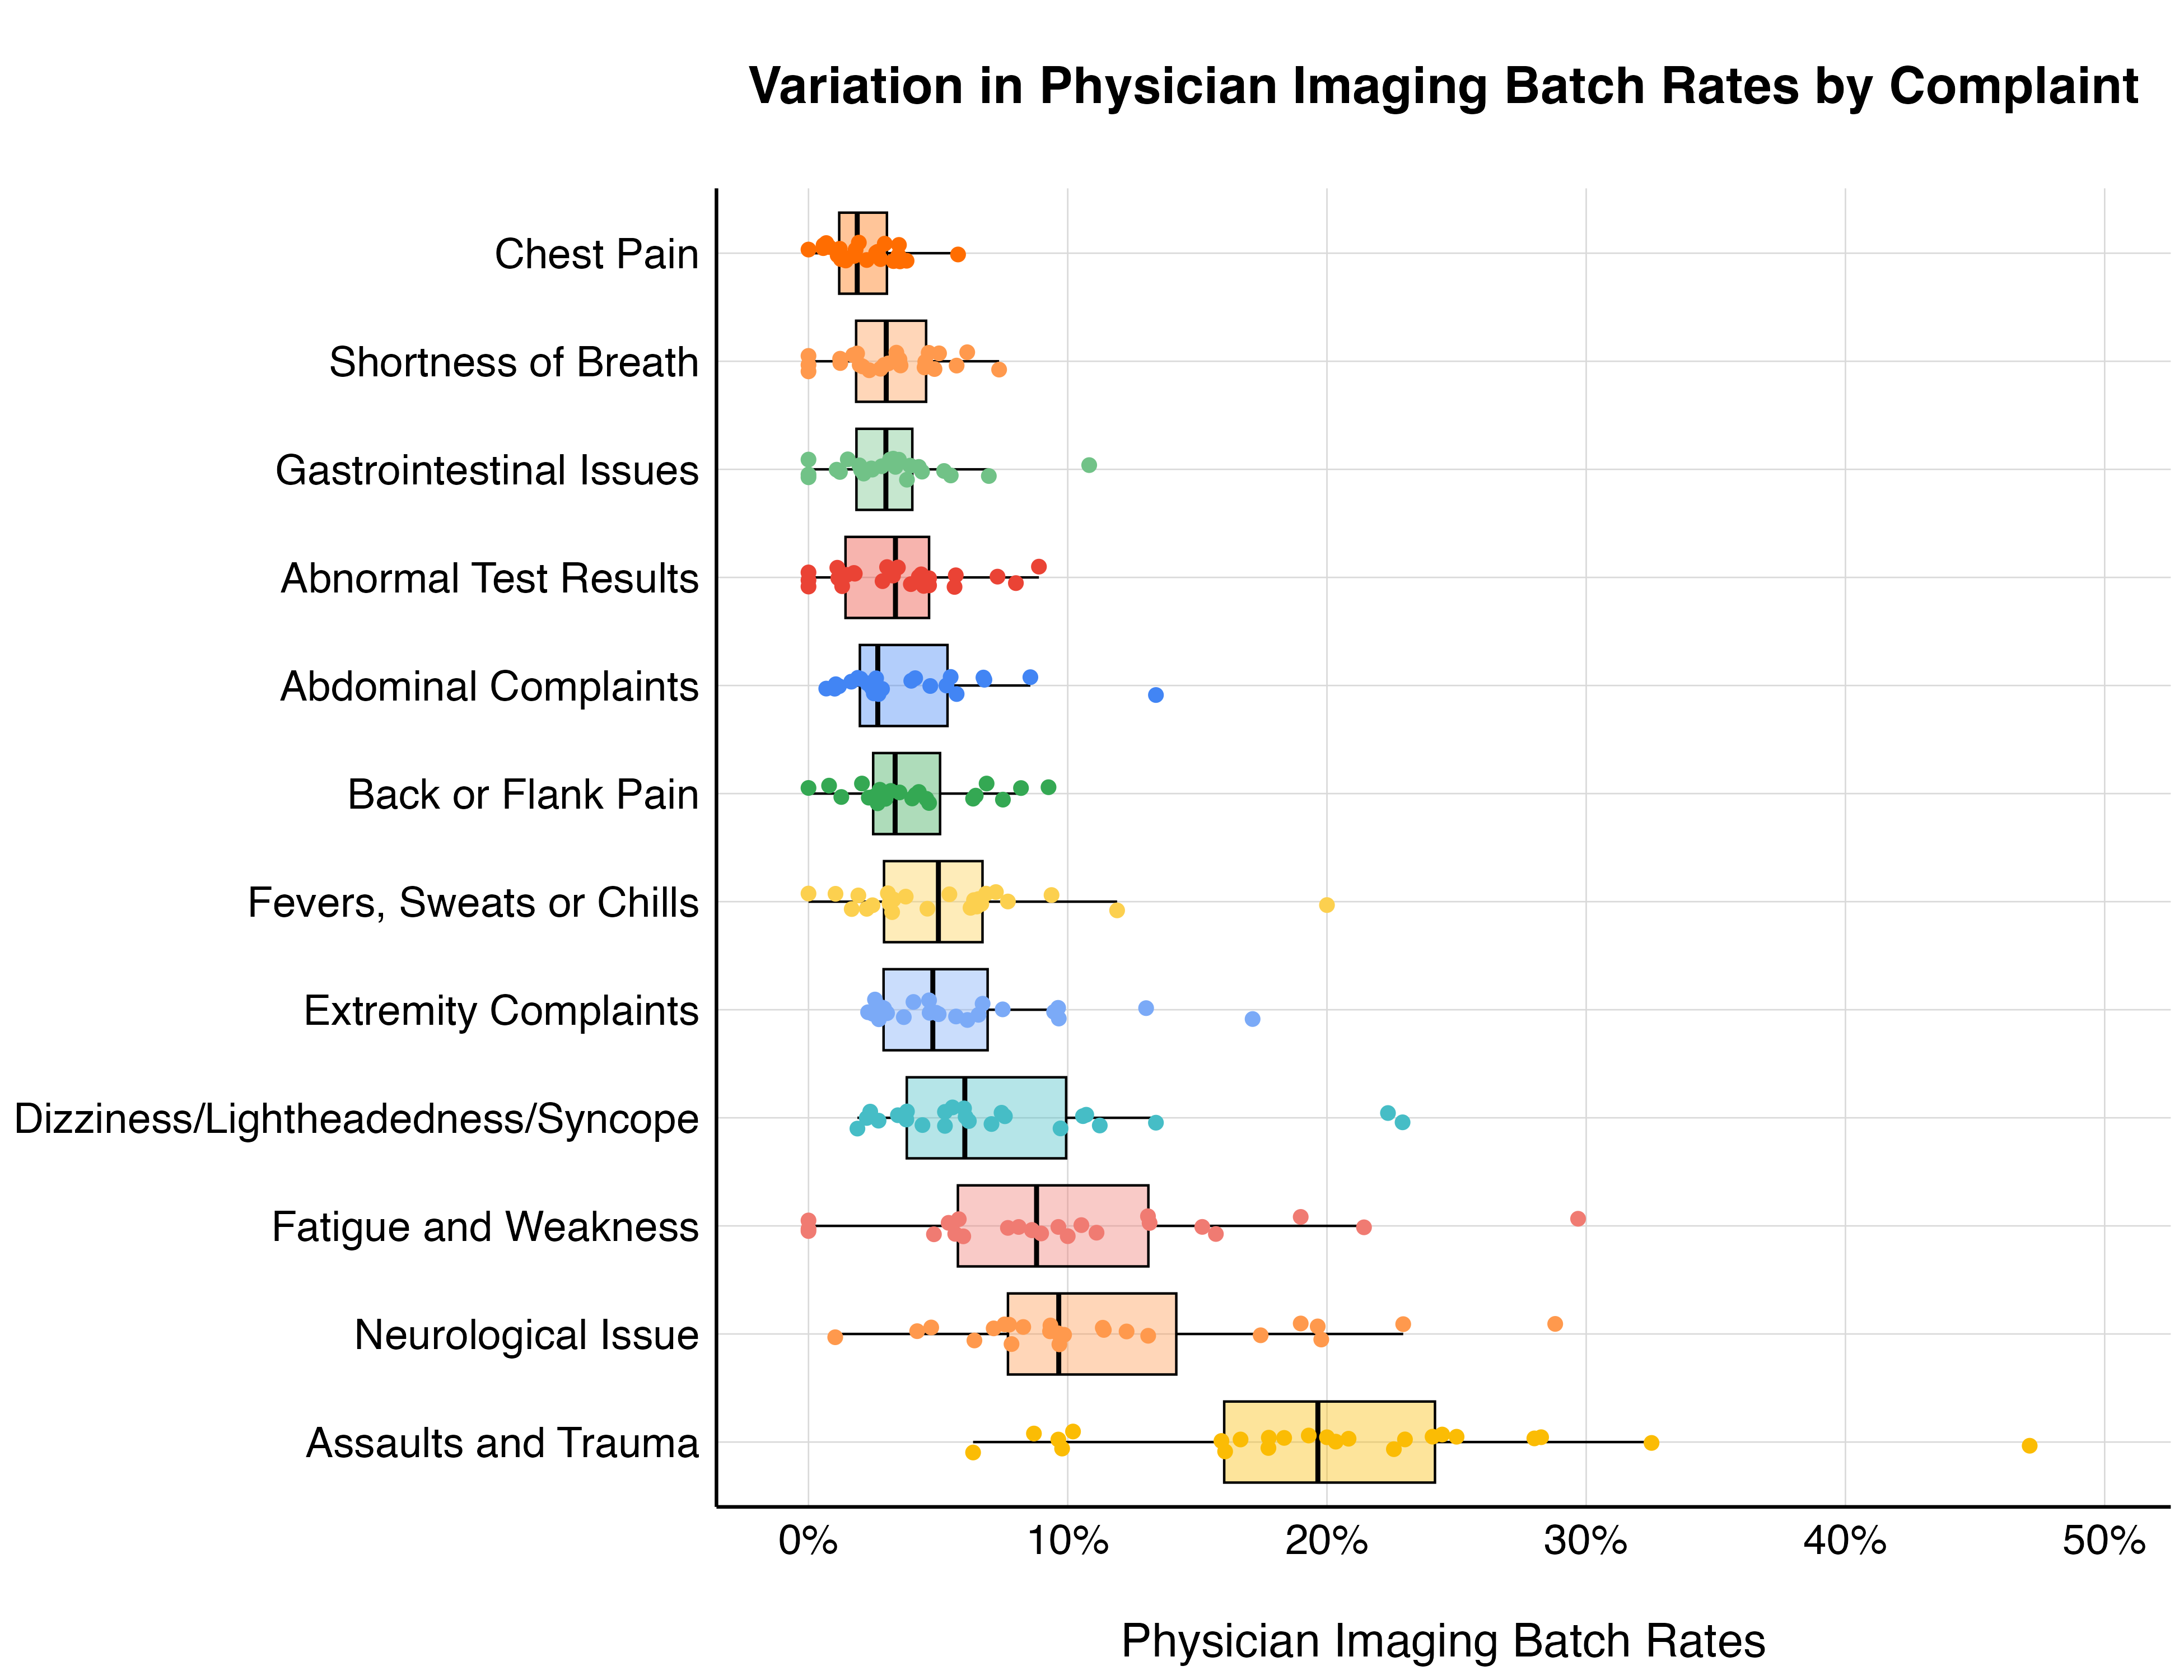
\includegraphics[width=4.25in]{../outputs/figures/Figure 1.png}
\begin{tablenotes}
\small
\item \textit{Figure \ref{fig:physician_batching} illuminates the marked differences among physicians in their propensity to batch-order diagnostic tests.}
\end{tablenotes}  
\end{figure}

\hyperref[table:first_stage]{Table } illustrates the ``first stage''
results, emphasizing the robust relevance of the instrument across
various controls. Being assigned to a \(10\)pp higher batch-tendency
physician is associated with a \(17.6\)pp increase in the probability of
having tests batch-ordered in the ED. The F-statistic is 21.6 when all
controls and fixed effects are included. The coefficient is greater than
one because all emergency visits are used to construct the tendency
instrument, while the first stage is calculated using the baseline
sample only.

\begin{table}[!htbp] \centering 
  \caption{Comparison of First Stage Estimates}
  \label{table:first_stage}
  \begin{tabularx}{5.5in}{Xccc} % 'X' for the first column and 'c' for the others
  \toprule
   & \multicolumn{3}{c}{Coeffecient} \\
  \cmidrule{2-4}
   & (1) & (2) & (3) \\
  \midrule
  Batch Tendency & 1.92$^{***}$ & 1.91$^{***}$ & 1.76$^{***}$ \\ 
   & (0.07) & (0.06) & (1.76) \\ 
  \textit{Day of Week-Time of Day FE} & $\checkmark$ & $\checkmark$ & $\checkmark$ \\
  \textit{Month of Year FE} & $\checkmark$ & $\checkmark$ & $\checkmark$ \\
  \textit{Complaint/Severity FE} & & $\checkmark$ & $\checkmark$ \\
  \textit{Laboratory Tests Ordered} & & & $\checkmark$ \\
  \midrule
  F Statistic & 9.55 & 17.86 & 21.59 \\ 
  N & 16,361 & 16,361 & 16,361 \\ 
  \bottomrule
  \end{tabularx}
  \begin{tablenotes}
  \small
  \item Estimates of the first stage for the baseline sample described in the text. Seasonality shift fixed effects include Year-Month and Hospital-Day of week-Hour of day fixed effects. Chief complaint comes from the cleaned complaint that the patient came in with at the initial encounter. Column 3 corresponds to the baseline controls. Robust standard errors are clustered at the physician level.
  \item $^{***} p < 0.001$, $^{**} p < 0.01$, $^{*} p < 0.05$.
  \end{tablenotes}
\end{table}

To estimate the reduced-form effects of being treated by a
batch-preferring physician, we estimate the following equation:

\begin{equation}
Y_i = \mu_0 + \mu_1 Tendency_{i,j}^{phys} + \gamma X_i + \nu_i
\end{equation}

This reduced form allows us to check the strength of our instrument. To
study the effects of test batching in the ED, we employ a multi-stage
approach using our baseline sample:

\begin{equation}
Tests_i = \alpha_0 + \alpha_1 Batched_i + \delta X_i + \eta_i
\end{equation}

\begin{equation}
Y_i = \beta_0 + \beta_1 Batched_i + \beta_2 Tests_i + \theta X_i + \varepsilon_i
\end{equation}

Where \(Tests_i\) is the number of imaging tests ordered, and \(Y_i\)
represents our patient outcomes of interest: length of stay and 72-hour
return with admission. \(X_i\) is the same set of control variables as
in the reduced-form approach. The \(Batched_i\) variable suffers from
potential endogeneity concerns. For example, unobserved injury severity
may correlate with both the need for multiple tests and patient
outcomes. To address this, we instrument \(Batched_i\) with the assigned
physician \(j\)'s underlying tendency to batch,
\(Tendency_{i,j}^{phys}\). We use a causal mediation analysis to
decompose the total effect of batching into its direct effect on
outcomes and its indirect effect through the number of tests ordered.
This approach employs bootstrapping to estimate confidence intervals for
the direct and indirect effects. We cluster standard errors at the
physician level to account for potential correlation in outcomes among
patients treated by the same physician, and to properly adjust for the
shared physician-level instrument across patients.

\hypertarget{identifying-assumptions}{%
\subsection{Identifying Assumptions}\label{identifying-assumptions}}

The reduced-form approach delivers an unbiased estimate of the causal
effect of being treated by a higher tendency to batch physician, since
assignment of patients to ED physicians is random, conditional on
seasonality and shift (``conditional independence''). The
residualization in equation (4) controls for more controls than required
to achieve quasi-random assignment; they are included for statistical
precision in measuring physician tendency to batch.

Our instrumental variable approach, which aims to recover the causal
effect of having diagnostic tests batch ordered, relies on three
additional assumptions: relevance, exclusion, and monotonicity. We
reported a strong first stage (i.e., relevance) at the end of the
previous Section. The exclusion restriction requires that the instrument
must influence the outcome of interest only through its effect on test
batching. This is perhaps our strongest assumption and is at its core,
untestable. However, several features of the ED setting suggest that
such violation may likely only have a small impact and may be less
concerning than in other health care settings. First, unlike in primary
care settings, where the patient and primary care provider have many
repeat encounters, the scope of what the emergency physician can do to
impact medium-term outcomes is limited and well-observed by the
researcher. Second, any violation of the exclusion restriction needs to
directly affect the specific outcome of interest. The channel by which
ED physicians can influence length of stay relative outcomes is likely
through testing and diagnosis. Nevertheless, we take this assumption
seriously and perform a placebo check in Section 5.2 as well as various
robustness checks in Section 6.

Finally, the monotonicity assumption is necessary for interpreting the
coefficient estimates obtained from the IV approach as Local Average
Treatment Effects (LATEs) if there are heterogeneous treatment effects.
It requires that any patient who is (not) batched by a sequencer
(batcher) would also (not) be batched by a batcher (sequencer)
physician. The literature leveraging the judges design typically
performs two informal tests for its implications. The first one provides
that the first stage should be weakly positive for all subsamples
(\citet{dobbie2018effects}). The second implication asserts that the
instrument constructed by leaving out a particular subsample has
predictive power over that same left-out subsample
(\citet{bhuller2020incarceration}). Appendix Table
\ref{tab:monotonicity} presents both of these tests in the two columns
for various subsamples of interest.

\hypertarget{sec:4}{%
\section{Results}\label{sec:4}}

\hypertarget{reduced-form-results}{%
\subsection{Reduced-Form Results}\label{reduced-form-results}}

In this section, we explore the causal influence of physician batch
tendency on total imaging volumne in the emergency department. We posit
that while batch tendency directly influences the practice of batch
ordering tests, both batch tendency and batch ordering are concurrently
influenced by a physician's testing inclination. Given that testing
inclination directly affects primary outcomes, we include it as a
control variable in our regression models to mitigate its confounding
effects.

To quantify a physician's testing inclination, we employ a similar
approach to that used in measuring physician batch tendency.
Specifically, we calculate the physician's residualized leave-out
average imaging test order rate, which serves as a proxy for their
propensity to order tests. It is important to note the strong positive
correlation between batch tendency and testing inclination, suggesting
that physicians with a higher propensity to test may also exhibit a
higher tendency to batch orders, potentially as a consequence of their
testing strategies. Neglecting to account for testing inclination could
lead to overestimated effects of batch tendency due to omitted variable
bias.

Reduced-form regression results in Table \ref{tab:reducedform} reveal
the effect the average total effect of batch tendency on the number of
distinct imaging tests ordered for our final sample. We hypothesize that
while batch ordering may streamline the testing process, resulting in a
quicker completion of a given number of tests, it simultaneously appears
to lead to an increase in the total number of tests ordered. The
increased testing volume, in turn, is associated with an extended LOS
and possibly lower rate of return with admission.

\begin{table}[!htbp] \centering 
  \caption{Reduced Form Results: Effect of Batch Tendency on the Number of Unique Imaging Tests Ordered}
  \label{table:reduced_form}
  \begin{tabularx}{5.5in}{Xccc} % 'X' for the first column and 'c' for the others
  \toprule
   & \multicolumn{3}{c}{Coeffecient} \\
  \cmidrule{2-4}
   & (1) & (2) & (3) \\
  \midrule
  Batch Tendency  & 4.543$^{***}$ & 1.11$^{***}$ & 1.11$^{*}$ \\ 
   & (0.532) & (0.124) & (0.447) \\
  \textit{Baseline Controls} &  $\checkmark$ & $\checkmark$ & $\checkmark$ \\ 
  \textit{Testing Inclination}  & & $\checkmark$ & $\checkmark$ \\
  \textit{Any Imaging Ordered} & & & $\checkmark$ \\ % Assumed to be included in (4)
  \midrule
  $R^2$ & 0.203 & 0.207 & 0.599 \\ 
  N & 16,361 & 16,361 & 16,361 \\ 
  \bottomrule
  \end{tabularx}
  \begin{tablenotes}
  \small
  \item Estimates of the reduced form for the baseline sample and baseline controls described in the text. Seasonality shift fixed effects include Year-Month and Hospital-Day of week-Hour of day fixed effects. Chief complaint comes from the cleaned complaint that the patient came in with at the initial encounter. Robust standard errors are clustered at the physician level.
  \item $^{***} p < 0.001$, $^{**} p < 0.01$, $^{*} p < 0.05$.
  \end{tablenotes}
\end{table}

\hypertarget{placebo-check}{%
\subsection{Placebo Check}\label{placebo-check}}

In this section we investigate whether the reduced-form effects observed
in Section 5.1 are due to differences in batch rates across providers or
due to other provider differences correlated with batch tendency. We
start by studying reduced-form effects among patients with complaints
that are never batched, as a ``placebo/falsification check.'' By way of
example, consider a patient who arrives at the ED with a urinary tact
infection---a condition for which patients rarely undergo imaging
testing. For such patients, we should expect to see no impact of batch
tendency only if high batching and low batching physicians do not
systematically differ in other dimensions of care relevant to patient
outcomes. Conversely, if we do find a reduced-form effect for these
patients, then high batch tendency physicians must systematically differ
from low batch tendency physicians in other dimensions of care, beyond
batching.

To that end, we restrict attention to ED visits for complaints where
batching occurs no more than 5 percent of the time (recall that our
baseline sample only includes complaints with a \(>5\) percent batching
rate). We estimate a reduced-form regression of each main outcome on
physician batch tendency for the subsample, following equation (6). The
results of this exercise are displayed in Appendix Table 1. They show
that in contrast to results for our main sample, the association between
physician tendency to batch and a given outcome is statistically
indistinguishable from zero and much smaller in magnitude for the
samples of patients who visit the ED with health conditions that are
rarely batched.

\hypertarget{instrumental-variables-results}{%
\subsection{Instrumental Variables
Results}\label{instrumental-variables-results}}

This section presents our causal analysis of batch ordering imaging
tests in the ED, focusing on its effects on resource utilization and
patient outcomes. Our analysis reveals nuanced impacts of batch
ordering, with significant implications for ED management and patient
care.

\hypertarget{effect-of-batch-ordering-on-imaging-tests-and-patient-outcomes}{%
\subsubsection{Effect of Batch Ordering on Imaging Tests and Patient
Outcomes}\label{effect-of-batch-ordering-on-imaging-tests-and-patient-outcomes}}

Table \ref{tab:combined_results} presents the results of our two-stage
least squares (2SLS) analysis and subsequent causal mediation analysis
for our analytical sample.

\begin{table}[!htbp]
\centering
\caption{Combined 2SLS and Causal Mediation Analysis Results}
\label{tab:combined_results}
\begin{threeparttable}
\begin{tabularx}{\textwidth}{Xcccc}
\toprule
& Number of Imaging Tests & Log LOS & 72-hr Return with Admission \\ \cmidrule(l){2-2} \cmidrule(l){3-3} \cmidrule(l){4-5}
\midrule
\multicolumn{5}{l}{\textit{2SLS Results}} \\
\\
Batched & 0.699** & -0.539 & -0.036 & \\
& (0.286) & (1.534) & (0.034) & \\
\\
  \textit{Baseline Controls} &  $\checkmark$ & $\checkmark$ & $\checkmark$ \\ 
  \textit{Testing Inclination} &  $\checkmark$ & $\checkmark$ & $\checkmark$ \\ 
  \textit{Imaging Ordered} & $\checkmark$ & $\checkmark$ & $\checkmark$ \\ 
\midrule
\multicolumn{5}{l}{\textit{Causal Mediation Analysis}} \\
\\
ACME & & 0.083*  [0.017, 0.15] & -0.003**  [-0.005, 0.00] \\
ADE &  & -0.565  [-3.608, 2.56] & -0.034  [-0.101, 0.03] \\
Total Effect &  & -0.481  [-3.549, 2.60] & -0.037  [-0.104, 0.03] \\
\bottomrule
\end{tabularx}
\end{threeparttable}
\end{table}

Our 2SLS estimates reveal a significant positive effect of batch
ordering on the number of imaging tests performed. Specifically, batch
ordering leads to an increase of 0.699 imaging tests (95\% CI: {[}0.138,
1.260{]}, p \textless{} 0.05) per patient encounter. This finding
confirms our hypothesis that batch ordering results in a higher volume
of diagnostic imaging compared to a sequential approach. The magnitude
of this effect suggests that for every 100 batch orders, approximately
70 additional imaging tests are performed that would not have occurred
under a sequential ordering strategy.

This excess in imaging tests can be attributed to the fundamental
difference between batch and sequential ordering approaches. In a
sequential approach, physicians can incorporate the information gained
from initial tests to inform decisions about subsequent testing,
potentially reducing unnecessary examinations. Batch ordering, by
contrast, commits to multiple tests upfront, without the benefit of this
stepwise information gain.

\hypertarget{mediation-analysis-imaging-volume-as-a-mediator}{%
\subsubsection{Mediation Analysis: Imaging Volume as a
Mediator}\label{mediation-analysis-imaging-volume-as-a-mediator}}

Our causal mediation analysis provides crucial insights into how the
increased imaging volume affects key patient outcomes. For length of
stay (LOS), we find a significant Average Causal Mediation Effect (ACME)
of 0.0834 (95\% CI: {[}0.0171, 0.15{]}, p \textless{} 0.1). This
positive ACME indicates that batch ordering indirectly extends ED stays
through increased testing. Notably, while the Average Direct Effect
(ADE) of batch ordering on LOS is negative (-0.565), it is not
statistically significant. These findings challenge the conventional
wisdom that batch ordering is a time-saving measure. While there may be
some efficiency gains in the testing process itself (as suggested by the
negative, albeit non-significant, ADE), these are more than offset by
the additional time required to perform and interpret the excess tests
generated by batch ordering. The net result is a tendency towards longer
patient stays in the ED.

Interestingly, our analysis of 72-hour return rates with admission
reveals a contrasting effect. We observe a small but statistically
significant negative ACME of -0.00274 (95\% CI: {[}-0.00550, 0.00{]}, p
\textless{} 0.05). This suggests that the increased imaging from batch
ordering may slightly reduce the probability of patients returning to
the ED within 72 hours and requiring admission. This finding indicates
that the ``shotgun'' approach of comprehensive initial testing may have
some benefits in terms of thorough patient evaluation, potentially
catching issues that might otherwise lead to return visits. These
results paint a nuanced picture of the impacts of batch ordering in the
ED. On one hand, it leads to increased resource utilization and longer
patient stays, which could strain ED capacity and potentially contribute
to overcrowding. On the other hand, it may result in more comprehensive
initial evaluations that slightly reduce short-term return visits.

The complexity of these findings underscores the need for careful
consideration in ED test ordering strategies. While batch ordering may
offer some benefits in terms of comprehensive initial evaluations, it
also carries significant costs in terms of resource utilization and
patient flow. ED managers and policymakers must weigh these trade-offs
carefully when developing guidelines for diagnostic testing. These
results also highlight the importance of considering both direct and
indirect effects when evaluating ED processes. The apparent efficiency
of batch ordering in the testing process itself may be misleading if one
does not account for the downstream consequences of increased test
volume. Given the varying impacts of batch ordering across different
outcomes, it is likely that the appropriateness of this practice may
depend on specific clinical scenarios or patient characteristics. To
further explore this possibility and provide more targeted insights for
ED management, we next conduct a subgroup analysis examining the effects
of batch ordering across different presenting complaints.

\hypertarget{subgroup-analysis-by-chief-complaint}{%
\subsubsection{Subgroup Analysis by Chief
Complaint}\label{subgroup-analysis-by-chief-complaint}}

Our subgroup analysis reveals important differences in the effects of
batch ordering across various presenting complaints, offering valuable
insights for optimizing diagnostic strategies in the ED. Table
\ref{tab:subgroup_analysis} presents these results.

\begin{table}[!htbp]
\centering
\caption{Subgroup Analysis Results by Chief Complaint}
\label{tab:subgroup_analysis}
\tiny
\begin{tabularx}{\textwidth}{Xcccccc}
\toprule
Chief Complaint & Batched Coefficient & ACME LOS & ADE LOS & ACME 72hr Return & ADE 72hr Return \\
\midrule
Extremity Complaints & 0.709* & 0.133* & 0.268 & -0.003 & -0.090 \\
 & (0.411) & [-0.030, 0.290] & [-3.640, 3.870] & [-0.012, 0.000] & [-0.214, 0.040] \\
 \\
Falls/MVCs/Trauma & 0.268 & 0.040 & -0.019 & -0.002 & 0.037 \\
 & (0.422) & [-0.103, 0.180] & [-3.109, 2.960] & [-0.009, 0.000] & [-0.055, 0.130] \\
 \\
Dizziness/Syncope & 1.572** & 0.193** & -1.353 & -0.011** & -0.023 \\
 & (0.701) & [0.015, 0.390] & [-4.043, 1.370] & [-0.025, 0.000] & [-0.270, 0.210] \\
 \\
Neurological Issue & 1.652 & 0.139 & -7.353 & 0.003 & -0.220 \\
 & (1.983) & [-0.242, 0.520] & [-16.602, 2.500] & [-0.020, 0.030] & [-0.987, 0.560] \\
 \\
Fatigue and Weakness & 0.793 & 0.072 & -0.286 & -0.002 & 0.010 \\
 & (0.686) & [-0.059, 0.220] & [-1.422, 0.940] & [-0.013, 0.000] & [-0.102, 0.120] \\
 \\
Fevers/Sweats/Chills & -0.181 & -0.025 & -1.086 & 0.002 & 0.061 \\
 & (0.858) & [-0.250, 0.200] & [-3.079, 1.000] & [-0.020, 0.030] & [-0.336, 0.430] \\
\bottomrule
\end{tabularx}
\end{table}

For extremity complaints, which range from minor injuries to potentially
severe conditions like deep vein thrombosis, batch ordering
significantly increases imaging volume (coefficient = 0.709, p
\textless{} 0.1) and indirectly extends ED length of stay (ACME = 0.133,
95\% CI: {[}-0.030, 0.290{]}, p \textless{} 0.1). However, this approach
also shows a trend towards reduced 72-hour returns (ACME = -0.003, 95\%
CI: {[}-0.012, 0.000{]}). These findings suggest that while batch
ordering for extremity complaints leads to more resource utilization and
longer stays, it may be preventing missed diagnoses of serious
conditions like fractures or vascular issues. For extremity complaints,
a targeted batch ordering approach may be beneficial. Clinicians should
consider batch ordering for patients presenting with symptoms suggestive
of more serious conditions (e.g., suspected fractures, vascular
compromises) or for those with complex medical histories. For minor
injuries or low-risk presentations, a sequential approach might be more
appropriate to balance resource use and patient flow.

Dizziness and syncope complaints demonstrate even stronger effects of
batch ordering. The significant increase in imaging volume (coefficient
= 1.572, p \textless{} 0.05) translates to longer ED stays (ACME =
0.193, 95\% CI: {[}0.015, 0.390{]}, p \textless{} 0.05) but also
significantly reduces 72-hour returns (ACME = -0.011, 95\% CI:
{[}-0.025, 0.000{]}, p \textless{} 0.05). This pattern likely reflects
the complex nature of these complaints, which can stem from benign
causes or indicate serious underlying conditions like stroke or cardiac
issues. For dizziness and syncope, the reduction in return visits
justifies a more liberal use of batch ordering. The potential to
identify serious underlying conditions outweighs the increased length of
stay. However, clinicians should still use clinical judgment to identify
low-risk patients (e.g., young patients with clear peripheral vertigo)
who might benefit from a more sequential approach.

For other complaint categories, including falls/trauma, neurological
issues, and general symptoms like fatigue or fever, the benefits of
batch ordering are less clear-cut. In these cases, the lack of
significant effects on return visits suggests that a more selective,
sequential approach to test ordering may be more appropriate. For these
complaints, we recommend a more individualized approach. Clinicians
should rely on thorough initial assessments and risk stratification to
determine the need for comprehensive imaging. Decision support tools
incorporating factors like patient age, comorbidities, and specific
symptoms could guide this process.

It is important to consider several key tradeoffs when implementing
batch ordering in the ED:

\begin{enumerate}
\def\labelenumi{\arabic{enumi}.}
\item
  Resource Utilization vs.~Patient Safety: While batch ordering
  increases resource use and ED length of stay, the potential reduction
  in return visits for certain complaints suggests improved diagnostic
  accuracy. EDs must weigh the upfront costs against the long-term
  benefits of preventing missed diagnoses and return visits.
\item
  ED Flow vs.~Comprehensive Care: Longer ED stays due to batch ordering
  could impact overall ED flow. However, for complaints like
  dizziness/syncope, this tradeoff appears justified by the reduced
  return rates. EDs should consider implementing parallel processes
  (e.g., rapid results reporting, streamlined discharge planning) to
  mitigate the impact on patient flow.
\item
  Cost Considerations: While our study doesn't directly address costs,
  the increase in imaging tests from batch ordering likely increases
  immediate healthcare costs. However, this may be offset by reduced
  costs from prevented return visits and earlier diagnosis of serious
  conditions. A comprehensive cost-benefit analysis would be valuable
  for future research.
\end{enumerate}

\hypertarget{robustness}{%
\subsection{Robustness}\label{robustness}}

\hypertarget{deifinition-of-batching}{%
\subsubsection{Deifinition of Batching}\label{deifinition-of-batching}}

The 2SLS results presented in the previous sections are robust to
several alternative specifications probing the key batching definition.
Our primary definition operationalizes batching as the ordering of
multiple diagnostic tests within a 5-minute window. This approach is
grounded in standard emergency medicine practices and offers a clear
distinction between batching and non-batching behaviors. To ensure the
robustness of our findings, we performed several sensitivity analyses.

\begin{enumerate}
\def\labelenumi{(\arabic{enumi})}
\item
  Variation in the Time Window for Batching: Firstly, we varied the time
  window for what constitutes a batch. The original 5-minute window was
  extended and contracted to understand its impact on the study's
  outcomes. Specifically, we considered scenarios where a batch is
  defined as two or more tests ordered within windows of 1 minute to 10
  minutes. This range allowed us to capture a broader spectrum of
  batching behaviors and test the sensitivity of our results to
  different batching definitions.
\item
  Refinement of Batching Definition: Secondly, we refined our batching
  definition based on the sequence and timing of test orders. In the
  initial analysis, if two tests were ordered upfront and another test
  ordered later, it was counted as a batch. We modified this definition
  to consider a set of tests as a batch only if all tests ordered during
  a patient encounter came from that initial batch order. This
  adjustment ensures that our batching definition more accurately
  reflects a comprehensive diagnostic effort at the outset of patient
  care, rather than incremental decision-making.
\end{enumerate}

The key finding from these robustness checks is the consistent impact of
batching on key outcomes across all variations. As seen in Appendix
Table 2 and 3, altering the time window for batching, whether narrowing
it to as little as 1 minute or expanding it to 10 minutes, did not
qualitatively change the results. Similarly, refining the definition of
batching to consider only those tests ordered in the initial batch also
had negligible impact on the study's main findings. These results lend
further credibility to our initial findings, demonstrating that our
conclusions about the impact of batching on patient outcomes in the ED
are not sensitive to the specific operational definition of batching.

\hypertarget{external-validity}{%
\subsubsection{External Validity}\label{external-validity}}

To assess the generalizability of our findings and ensure their
robustness, we conducted an additional analysis using data from the
Emergency Department of Massachusetts General Hospital (MGH). This
high-volume ED sees approximately 110,000 patient encounters annually,
providing a diverse and extensive dataset for comparison. Our analysis
utilized 12 months of ED visit data from MGH, encompassing a wide range
of patient presentations, diagnoses, and outcomes. This dataset provides
a valuable contrast to our primary study site, offering insights into
how batch ordering practices and their effects may vary in a different
clinical environment.

It is important to note that the MGH ED does not employ the same
quasi-random assignment of patients to physicians as our primary study
site. This difference in patient allocation necessitated an alternative
analytical approach. To address potential selection bias and create a
fair comparison between batched and non-batched cases, we employed a
propensity score matching technique, which involves:

\begin{itemize}
\item
  Score Calculation: We calculated propensity scores for each patient
  encounter based on key variables including: Chief complaint, Severity
  (as measured by the Emergency Severity Index or an equivalent triage
  score), Time of day, Day of week, and Patient demographics (age,
  gender).
\item
  Matching: Using these propensity scores, we matched patients who
  received batch-ordered imaging tests with those who did not. We
  employed a nearest-neighbor matching algorithm with a caliper width of
  0.2 standard deviations of the logit of the propensity score, which is
  widely accepted in the literature as a balance between matching
  quality and number of matched pairs.
\item
  Balance Checking: After matching, we conducted balance checks to
  ensure that the matched groups were comparable across all covariates
  used in the propensity score calculation. This included visual
  inspection of covariate distributions and statistical tests (e.g.,
  standardized mean differences) to confirm adequate balance.
\item
  Outcome Comparison: With our matched sample, we compared outcomes
  between the batched and non-batched groups, focusing on the same key
  metrics as our primary analysis: length of stay, number of imaging
  tests performed, and 72-hour return rates with admission.
\end{itemize}

This approach allows us to estimate the effect of batch ordering in a
setting where randomization is not feasible, by creating comparable
groups of batched and non-batched cases. While this method cannot fully
replicate the strengths of our primary quasi-experimental design, it
provides a valuable check on the external validity of our findings. By
comparing the results from this analysis to our primary findings, we can
assess whether the effects of batch ordering on ED outcomes are
consistent across different hospital settings and patient populations.
This comparison enhances the generalizability of our conclusions and
provides additional context for our recommendations on ED imaging
practices. The results of this external validation analysis are
presented in Appendix Table XX.

\hypertarget{conclusion}{%
\section{Conclusion}\label{conclusion}}

This study provides empirical evidence on the impacts of batch ordering
imaging tests in emergency departments, illuminating the trade-offs
between comprehensive initial assessments and efficient resource
utilization. Our findings, derived from a quasi-experimental design
leveraging physician practice variation, align closely with our
theoretical model of ED decision-making. We demonstrate that batch
ordering, while leading to more thorough initial evaluations, results in
increased resource use and longer ED stays.

The fundamental tension we uncover is between the information gain
approach of sequential testing and the comprehensive but potentially
excessive nature of batch ordering. Our results indicate that batch
ordering leads to approximately 70 additional imaging tests per 100
patient encounters compared to a sequential approach. This substantial
increase in testing volume translates to longer ED stays but also
slightly reduced 72-hour return rates with admission. These findings
underscore the complex decision-making environment in EDs, where
physicians must balance the need for thorough diagnostics against
operational efficiency and patient flow.

Importantly, our subgroup analysis reveals significant heterogeneity in
the effects of batch ordering across different presenting complaints.
For conditions with high diagnostic uncertainty or potential for serious
underlying issues, such as dizziness or syncope, the benefits of
comprehensive initial testing may outweigh the costs of increased
resource utilization. Conversely, for more straightforward
presentations, a sequential, information gain approach appears more
appropriate. This variation in effects emphasizes the need for nuanced,
complaint-specific approaches to test ordering in emergency settings.

Our results have significant implications for ED management and health
policy. They suggest that a one-size-fits-all approach to diagnostic
testing in the ED is suboptimal. Instead, ED managers and policymakers
should consider implementing targeted batch ordering strategies that
account for the specific nature of patient presentations and the
relative risks of missed diagnoses versus overcrowding and resource
strain. Future research should focus on developing and validating
decision support tools that can guide clinicians in choosing between
batch and sequential ordering based on patient-specific factors and
presenting complaints.

In conclusion, this study contributes to our understanding of ED
operations by quantifying the causal impacts of different diagnostic
testing strategies. By highlighting the nuanced trade-offs involved in
batch ordering, we provide a foundation for more informed
decision-making in emergency care. As healthcare systems continue to
grapple with the dual challenges of providing high-quality care and
managing limited resources, insights from studies like this one will be
crucial in shaping evidence-based policies and practices in emergency
medicine.

\newpage

% Appendix here
% Options are (1) APPENDIX (with or without general title) or
%             (2) APPENDICES (if it has more than one unrelated sections)
% Outcomment the appropriate case if necessary
%
% \begin{APPENDIX}{<Title of the Appendix>}
% \end{APPENDIX}
%
%   or
%
% \begin{APPENDICES}
% \section{<Title of Section A>}
% \section{<Title of Section B>}
% etc
% \end{APPENDICES}


% Acknowledgments here
\ACKNOWLEDGMENT{}

\bibliographystyle{informs2014}
\bibliography{references.bib}



\end{document}
